
%\begin{frame}
\frametitle{Содержание} % Table of contents slide, comment this block out to remove it
\tableofcontents % Throughout your presentation, if you choose to use \section{} and \subsection{} commands, these will automatically be printed on this slide as an overview of your presentation
\end{frame}

\section{Введение}
\subsection{Язык программирования Java}
\begin{frame}
	\frametitle{\insertsection} 
	\framesubtitle{\insertsubsection}
	\textit{Java} - строго типизированный объектно-ориентированный язык программирования, разработанный 
	компанией Sun Microsystems. Приложения Java обычно транслируются в специальный байт-код, поэтому 
	они могут работать на любой компьютерной архитектуре, с помощью \textbf{виртуальной Java-машины}.
\end{frame}



% Streams
\subsection{Интерфейс потоков объектов}
\begin{frame}
\frametitle{\insertsection} 
\framesubtitle{\insertsubsection}
% Фича Java 8
% Ленивость
% Функциональный стиль
\begin{itemize}
	\item Java 8 - появление анонимных функций и \textit{java.util.stream}
	\item \textit{java.util.stream} - набор классов и интерфейсов для упрощения обработки последовательностей элементов с помощью функций высших порядков
	\inputminted{java}{code/StreamsExample.java}
	\item Аналоги в других языках - LINQ в C\#, коллекции Scala
\end{itemize}
\end{frame}
\subsection{Интерфейс потоков объектов. Пример.}
\begin{frame}
\frametitle{Java Stream API. Пример использования} % Table of contents slide, comment this block out
Задача - фильтровать, сортировать, преобразовать. Показать как это сделать при помощи циклов
\end{frame}
\begin{frame}
	\frametitle{\insertsection} 
	\framesubtitle{Задача}
	Найти имена людей, чей возраст меньше 18 лет, отсортировав по возрасту
\end{frame}
\begin{frame}
\inputminted{java}{code/CyclesUsage.java}
\end{frame}
\begin{frame}
\frametitle{Java Stream API. Пример использования} % Table of contents slide, comment this block out
Задача - фильтровать, сортировать, преобразовать. Показать как это сделать при помощи циклов
\end{frame}
\begin{frame}
\inputminted{java}{code/StreamUsage.java}
\end{frame}
\subsection{Интерфейс потоков объектов. Реализация}
\begin{frame}
\frametitle{Части цепочки вычислений} % Table of contents slide, comment this block out
\begin{itemize}
	\item \textbf{Источник объектов}. Например, массив, коллекция, функция генератор, потоки ввода/вывода и другие.
	\inputminted{java}{code/Producer.java}
	\item \textbf{Промежуточные операции}, которые преобразуют поток объектов.
	\begin{itemize}
		\item Без состояния
		\inputminted{java}{code/Stateless.java}
		\item С состоянием
		\inputminted{java}{code/Stateful.java}
	\end{itemize}
	\item \textbf{Завершающая операция}. Операция которая завершает цепочку, выполняя какое-либо действие над объектами внутри потока.
	\inputminted{java}{code/Termination.java}
\end{itemize}
\end{frame}

\begin{frame}
\frametitle{\insertsection} 
\framesubtitle{\insertsubsection}
Реализация библиотеки активно использует Spliterator. Это расширенная версия привычного итератора с некоторыми расширениями:
\begin{itemize}
	\item Имеет операцию split - то есть позволят разделить оставшееся множество объектов на две непересекающиеся части, которые можно обработать параллельно.
	\item Имеет набор характеристик:
	\begin{itemize}
		\item ORDERED - упорядоченность
		\item DISTINCT - все элементы различны (относительно equals)
		\item SORTED - элементы отсортированы
		\item SIZED - размер известен
		\item NONNULL, IMMUTABLE, CONCURRENT, SUBSIZED
	\end{itemize}
\end{itemize}
\end{frame}
\begin{frame}
\frametitle{\insertsection} 
\framesubtitle{\insertsubsection}
\begin{itemize}
	
	\item Существуют расширения $java.util.stream$ - StreamEx, jOOL. Эти библиотеки совместимы со стандартной реализацией, расширяя стандартные интерфейсы.
\end{itemize}
\end{frame}


% Debugger
\subsection{Отладчик}
\begin{frame}
\frametitle{Функции отладчика} % Table of contents slide, comment this block out to remove it
\begin{itemize}
	\item Отладчик - компьютерная программа, предназначенная для поиска ошибок в других программах.
	\item JDPA - инфраструктура для отладки Java приложения. Содержит набор интерфейсов и протоколов:
	\begin{itemize}
		\item JVM TI - Java VM Tool Interface - описывает сервисы, которая предоставляет виртуальная машина для отладки.
		\item JDWP - Java Debug Wire Protocol - протокол общения между отладчиком и виртуальной машиной. 
		\item JDI - Java Debug Interface - высокоуровневая Java библиотека для взаимодействия с виртуальной машиной.
	\end{itemize}
\end{itemize}
\end{frame}
\begin{frame}
\frametitle{\insertsection} 
\framesubtitle{\insertsubsection}
\begin{itemize}
	\item JDB (java debugger) - простой command-line отладчик для java. Поставляется с JDK. Предоставляет примитивные операции:
	\begin{itemize}
		\item Подключиться к виртуальной машине (возможно, удаленной)
		\item Добавить точку останова
		\item Показать список потоков
		\item ...
	\end{itemize}
	jdb является достаточно примитивной демонстрацией возможностей JDPA (Java Platform Debugger Architecture)
	\item Отладчики внутри среды разработки - IntelliJ IDEA, Eclipse, NetBeans и т.д. Они так же 
	используют JDPA, но активнее чем JDB
\end{itemize}
\end{frame}

\begin{frame}
\frametitle{\insertsection} 
\framesubtitle{\insertsubsection}
JDPA - инфраструктура для отладки Java приложения. Содержит набор интерфейсов и протоколов:
\begin{itemize}
	\item JVM TI - Java VM Tool Interface - описывает сервисы, которая предоставляет виртуальная машина для отладки. (TODO: сказать про примеры)
	\item JDWP - Java Debug Wire Protocol - протокол общения между отладчиком и виртуальной машиной. (TODO: сказать про абстракцию)
	\item JDI - Java Debug Interface - высокоуровневая Java библиотека для взаимодействия с виртуальной машиной. (сказать про зеркала реальных объектов)
\end{itemize}
\end{frame}

\begin{frame}[noframenumbering]
\frametitle{\insertsection} 
\framesubtitle{\insertsubsection}
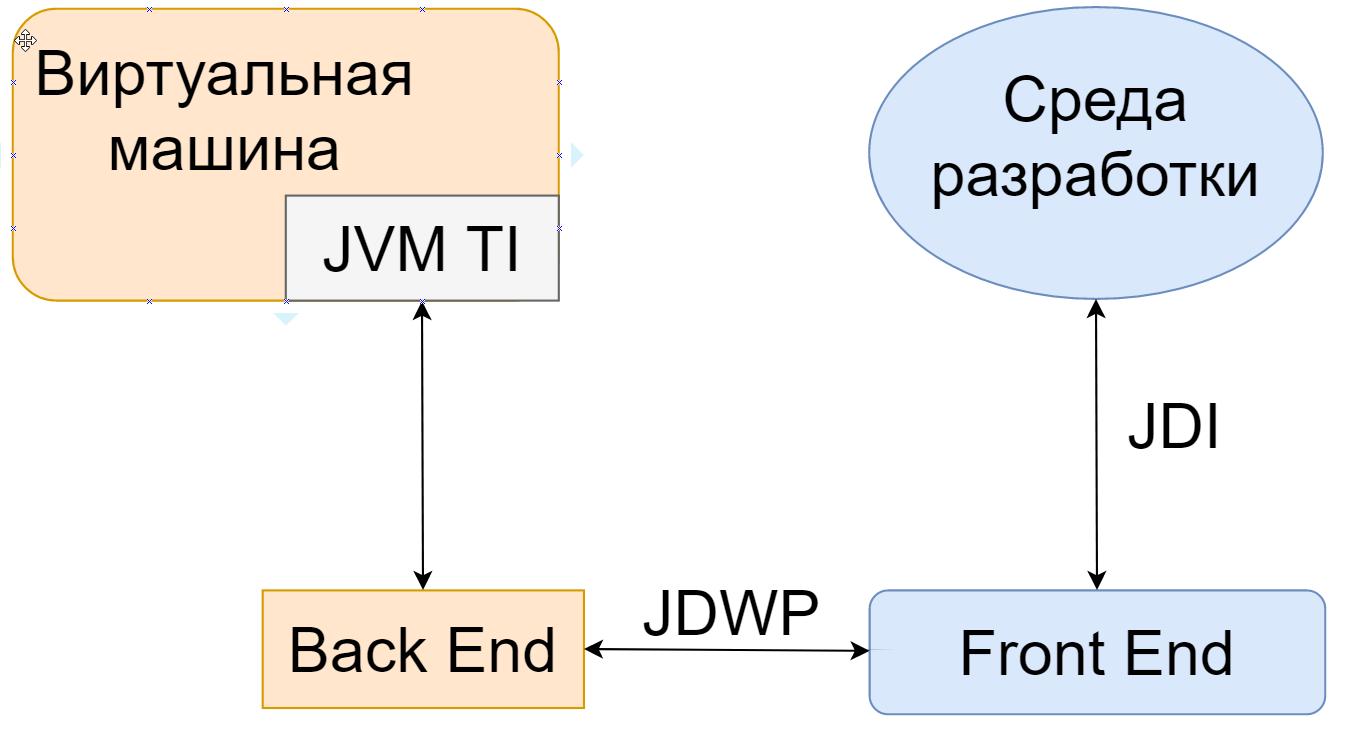
\includegraphics[scale=0.315]{img/jdpa.png}
\end{frame}

% Stream debugging
\section{Отладка потоков объектов}
\subsection{Поддержка со стороны сред разработки}
\begin{frame}
\frametitle{Сравнение отладки императивного кода и Stream API} % Table of contents slide, comment this block out to remove it
TODO: Построить таблицу, показать как можно, и как нет в обоих случаях
\end{frame}

\subsection{Проблемы}
\begin{frame}
\frametitle{\insertsection} 
\framesubtitle{\insertsubsection}
Недостатки отладки интерфейса потоков объекта в сравнении с обычными управляющими структурами
\begin{itemize}
	\item Отсутствие знаний о промежуточных результатах вычислений 
	\item Нетривиальная последовательность исполнения
	\item Отсутствие информации о трансформации объектов
	\item Простые стеки вызовов
	\item Отладка исключительных ситуаций % ?
\end{itemize}
\end{frame}

\subsection{Как сейчас можно отладить поток объектов}
\begin{frame}
\frametitle{\insertsection} 
\framesubtitle{\insertsubsection}
\begin{itemize}
	\item Точки останова (с условием)
	\item Последовательное исполнение
	\item При помощи метода peek
	\item Автоматическая конвертация в код с обычными управляющими структурами и отладка этого кода
	\item Частичное исполнение и сохранение во временную коллекцию (не во всех средах разработки)
\end{itemize}
\end{frame}

\subsection{Пример использования интерфейса потоков в проекте с открытым кодом}
\begin{frame}
\frametitle{\insertsection} 
\framesubtitle{\insertsubsection}
\inputminted{java}{code/Hard.java}
\end{frame}


\section{Цель}
\begin{frame}
	\frametitle{\insertsection} 
	\framesubtitle{\insertsubsection}
	\textbf{Цель}: Расширить возможности отладчика для поиска ошибок при использовании библиотек с функциями высшего порядка.
	
	\vspace{10px}
	\textbf{Задачи:}
	\begin{enumerate}
		\item Распознавание вызова Stream API возле текущей позиции отладчика.
		\item Построение промежуточных состояний между вызовами в цепочке.
		\item Нахождение переходов между состояниями.
		\item Визуализация объектов внутри состояний и переходов для них.
	\end{enumerate}
\end{frame}

\subsection{Существующие решения}
\begin{frame}
\frametitle{\insertsection} 
\framesubtitle{\insertsubsection}
Существует расширение для отладчика Visual Studio для C\# - OzCode. Одна из его функций - отладчик для LINQ
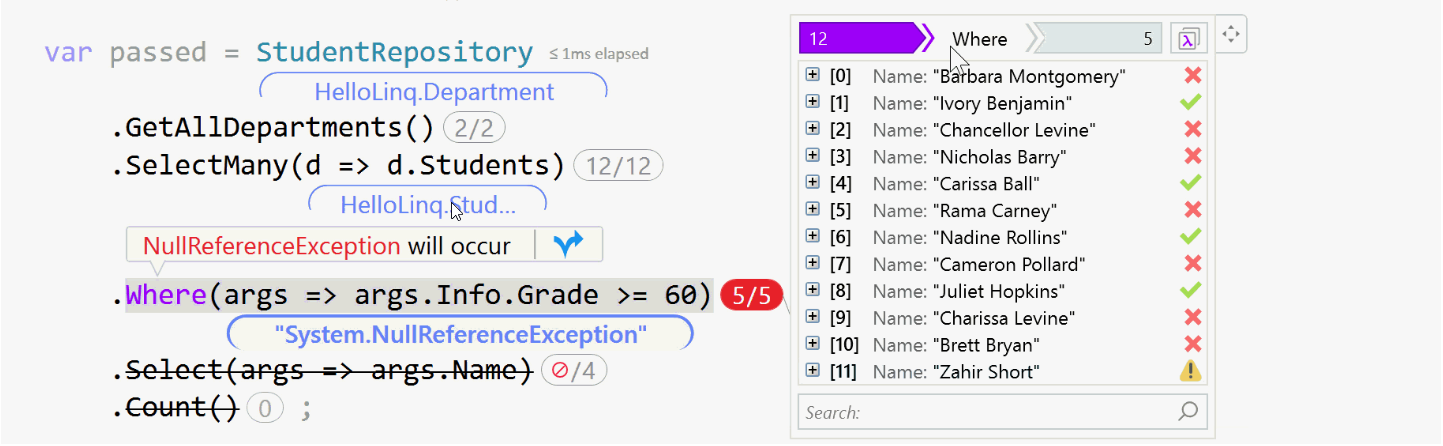
\includegraphics[scale=0.35]{img/ozcode.png}
\end{frame}

\subsection{Особенности OzCode}
\begin{frame}
\frametitle{\insertsection} 
\framesubtitle{\insertsubsection}
\begin{itemize}
	\item Работает с LINQ (язык интегрированных запросов), реализация которого отлична от реализации интерфейса потоков в Java
	\item Позволяет увидеть трансформации объектов и промежуточные результаты
	\item Закрытый исходный код
	\item Платный
	\item Только для отладчика Visual Studio
\end{itemize}
\end{frame}


\section{Решение}
\subsection{Гарантии, предоставляемые библиотекой}
\begin{frame}
\frametitle{\insertsection} 
\framesubtitle{\insertsubsection}
\begin{itemize}
	\item Поток объектов ленивый. Это значит, что объекты не из источника будут браться только когда выполняется терминальная операция и ей нужен объект.
	\item Это исключает ситуации, когда из каких-то промежуточных операций требовались объекты, но затем не использовались
	\item Но это не исключает, что некоторым промежуточным операциям потребуется прочитать более одного объекта, чтобы вернуть один. (см sorted, distinct, и др)
	\item Следствие: нет вызова терминальной операции - нет вычислений
\end{itemize}

\end{frame}
\subsection{Требования к пользовательскому коду}
\begin{frame}
\frametitle{\insertsection} 
\framesubtitle{\insertsubsection}
\begin{itemize}
	\item Операции над объектами не могут модифицировать объект - источник (если он есть)
	\item Функции над объектами в потоке не должны иметь состояния (в большинстве случаев)
\end{itemize}
\end{frame}
\subsection{Ограничения и особенности}
\begin{frame}
\frametitle{\insertsection} 
\framesubtitle{\insertsubsection}
Потоки объектов можно присваивать в промежуточные переменные.

\inputminted{java}{code/VariableAssign.java}
\end{frame}

\subsection{Метод peek}
\begin{frame}
\frametitle{\insertsection} 
\framesubtitle{\insertsubsection}
Интерфейс Stream для отладочных целей определяет метод peek.
\inputminted{java}{code/StreamWithPeeks.java}
\end{frame}

\begin{frame}[noframenumbering]
\frametitle{\insertsection} 
\framesubtitle{\insertsubsection}
\fboxsep=0pt
\noindent
	\begin{minipage}[t]{0.48\linewidth}
		Информация, которую можно извлечь:
		\begin{itemize}
			\item Последовательность прохождения объектов через цепочку вызовов
			\item Результат фильтрации
			\item sorted имеет состояние и требует выполнить весь поток до своего вызова
			\item Преобразования объектов
		\end{itemize}
	\end{minipage}
	\hfill%
		\begin{minipage}[t]{0.48\linewidth}
			Результат вызова:
			\inputminted{text}{code/peekResults.txt}
		\end{minipage}
\end{frame}

\subsection{Обобщение}
\begin{frame}
\frametitle{\insertsection} 
\framesubtitle{\insertsubsection}
Такой подход можно обобщить.
Для любого промежуточного вызова запомним объекты перед и после вызова.
\begin{align*}
	&.peek(x \rightarrow store(x, time)) \\
	&.call(...)\\
	&.peek(z \rightarrow \{time.increment()\})\\
	&.peek(y \rightarrow store(y, time))
\end{align*}

В результате получим два множества $Before = \{(t_i, x_i)\}, After = \{(t_i, y_i)\}$. 

Чтобы найти переходы достаточно построить \textbf{отображения}
\begin{align*}
	(t_i, x_i) \rightarrow List[(t_j, y_j)], \ \forall (t_i, x_i) \in Before \\
	(t_i, y_i) \rightarrow List[(t_j, x_j)], \ \forall (t_j, y_j) \in After
\end{align*}

\end{frame}

\subsection{Пример}
\begin{frame}
\frametitle{\insertsection} 
\framesubtitle{\insertsubsection}
Рассмотрим в качеству примера вызов:
\inputminted{java}{code/FlatMapFactorizeExample.java}
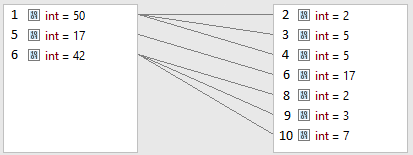
\includegraphics[scale=0.8]{img/flatMapExample.png}

Решая такие же задачи и для остальных методов, сможем получить отображения для всех. (с возможностью легко расширить набор поддерживаемых методов, например, поддержав сторонние библиотеки)
\end{frame}

\subsection{Исключения}
\begin{frame}
\frametitle{\insertsection} 
\framesubtitle{\insertsubsection}
Подойдет ли такое решение абсолютно для всех вызовов?
\begin{itemize}
	\item Нет, но почти для всех этого достаточно.
	\item Проблемы возникают с операциями, обладающими \textbf{состоянием}.
	\item Но таких вызовов немного и для каждого из них можно придумать решение.
\end{itemize}
\end{frame}

\subsection{Вычисление}
\begin{frame}
\frametitle{\insertsection} 
\framesubtitle{\insertsubsection}
Выполнение кода трассировки.
\begin{enumerate}
	\item Построить выражение с дополнительными вызовами peek и обработкой собранной информации.
	\item Скомпилировать новый класс, в котором будет код, вычисляющий выражение.
	\item Загрузить его в виртуальную машину и выполнить.
	\item Получить результат вычислений и интерпретировать его.
\end{enumerate}
\end{frame}

\begin{frame}[noframenumbering]
\frametitle{\insertsection} 
\framesubtitle{\insertsubsection}
Чтобы вычислить выражение для отслеживания исполнения цепочки потоков объектов нужно определить класс, а так же учесть следующие особенности
\begin{itemize}
	\item Поля и методы этого класса.
	
	\item Расположение класса: пакет, объемлющий класс.
	
	\item Доступ к полям и методам объемлющего класса.

	\item Доступ к приватным членам класса из лямбд и анонимных классов.

	\item Минимизация дальнейших обращений к виртуальной машине.
\end{itemize}

\inputminted{java}{code/EvalClass.java}
\end{frame}


\section{Дополнительно}
\begin{frame}
\frametitle{\insertsection} 
\framesubtitle{\insertsubsection}
Описанный подход позволяет исполнять код "в песочнице". Поэтому можем собирать дополнительную информацию.
\end{frame}

\subsection{Исключения}
\begin{frame}
\frametitle{\insertsection} 
\framesubtitle{\insertsubsection}
Определение вызова и объекта, на котором произошло исключение.
\inputminted{java}{code/Exceptions.java}
\end{frame}


\subsection{Промежуточные состояния итераторов}
\begin{frame}
\frametitle{\insertsection} 
\framesubtitle{\insertsubsection}
\inputminted{java}{code/Spliterator-props.java}
\end{frame}

\begin{frame}
\frametitle{\insertsection} 
\framesubtitle{\insertsubsection}
\inputminted{java}{code/Spliterator-props.java}
Вывод в Java 8: 123

Вывод в Java 9:

Причина - использование характеристик итераторов
\end{frame}


\section{Что сделано}
\begin{frame}
\frametitle{Что сделано}
TODO: простой трассирующий плагин
\end{frame}

\begin{frame}
\frametitle{\insertsection} 
\framesubtitle{\insertsubsection}
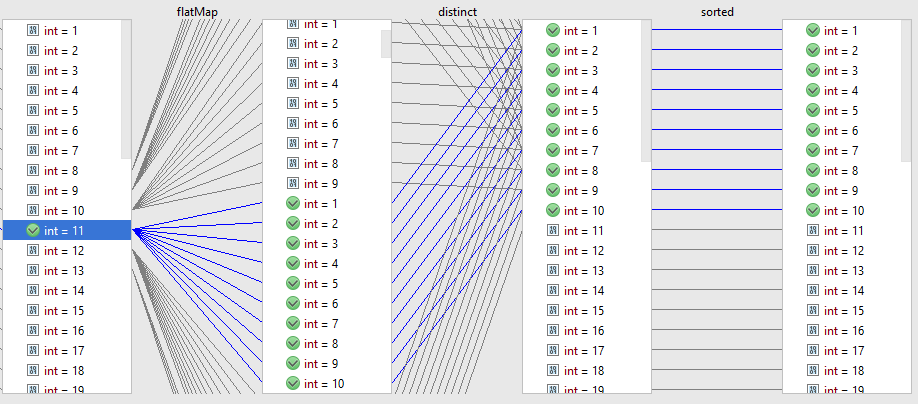
\includegraphics[scale=0.5]{img/trace-view.png}
\end{frame}


\section{Что ещё нужно сделать}
\begin{frame}
\frametitle{Что будет сделано}
TODO: Брейкпоинты, evaluation, etc
\end{frame}
